\section{Network layer}

\begin{definition}
    {Autonomous Systems (ASes)}

    Each system is:
    \begin{itemize}
        \item assigned a collection of IP addresses
        \item controlled by a company or organization
        \item responsible for routing to addresses within or outside the AS
        \item connected to each other at \textbf{Internet Exchange Points}
    \end{itemize}
\end{definition}

\begin{definition}
    {Networks}

    A \textbf{shared medium} with at least 2 interfaces attached to it.
    \begin{itemize}
        \item A switch connected to multiple computers is a network
        \item A router connected to other routers is a network
    \end{itemize}
    Hosts inside the network can directly communicate with each other.
\end{definition}

\sectionbar{M05-L01}

\subsection{Forwarding and routing}

\begin{definition}
    {Forwarding vs Routing}

    \textbf{Forwarding} is the process of moving packets from a router's input to the appropriate output.

    \textbf{Routing} is the process of determining the path that packets take from source to destination.
\end{definition}

\begin{definition}
    {Network layer components}

    \textbf{Data plane} is responsible for forwarding packets.

    \textbf{Control plane} is responsible for routing.
\end{definition}

% \begin{knBox}
%     {IPv4 and IPv6 datagram header}
%     ...
% \end{knBox}

% \begin{knBox}
%     {Subnet}

% \end{knBox}

\begin{definition}
    {IPv4 Addressing}

    An IPv4 address is a 32-bit number represented in dotted decimal notation as \texttt{a.b.c.d} where each of \texttt{a}, \texttt{b}, \texttt{c}, and \texttt{d} are 8-bit numbers (0-255).

    The bits are separated into \textbf{Network address} and \textbf{Host address}, based on the network's configuration (see below sections)

    \begin{itemize}
        \item Host address identifies a specific device on the network.
        \item All 0s $\to$ represent the network
        \item All 1s $\to$ represent broadcast to all hosts on the network
    \end{itemize}
\end{definition}

\begin{theorem}
    {Netmask and network bit size}

    \textbf{Network bit size} indicates the number of leading bits are used for the Network ID.

    A \textbf{netmask} is a 32 bit number with the first \texttt{x} bits set to 1 (where \texttt{x} is the network bit size) and the remaining bits set to 0.

    Routers only care about the network part. To find the \textbf{network address}, perform a \textbf{bitwise AND} between the IP address and the netmask.
\end{theorem}

\begin{knBox}
    {Classful addressing}
    Allocate IPv4 addresses based on leading bits (binary):

    \begin{tabular}{l|l|l}
        \textbf{Class}   & \textbf{Leading bits} & \textbf{Network bit size} \\
        \hline
        A                & 0                     & 8                         \\
        B                & 10                    & 16                        \\
        C                & 110                   & 24                        \\
        D (multicast)    & 1110                  & 32                        \\
        E (experimental) & 1111                  & 32                        \\
    \end{tabular}

    This is straight forward but \textbf{wasteful} as networks usually have too much or too little IP addresses

    \tcblower

    \begin{itemize}
        \item \texttt{12.0.0.0} $\implies$ Leading bits \texttt{00001100} $\to$ Class A, Network ID: \texttt{12}, Host ID: \texttt{0.0.0}
        \item \texttt{172.16.0.0} $\implies$ Leading bits \texttt{10101100} $\to$ Class B, Network ID: \texttt{172.16}, Host ID: \texttt{0.0}
        \item \texttt{192.168.1.0} $\implies$ Leading bits \texttt{11000000} $\to$ Class C, Network ID: \texttt{192.168.1}, Host ID: \texttt{0}
    \end{itemize}
\end{knBox}

\begin{definition}
    {Classless Inter-Domain routing Address (CIDR)}

    Allows \textbf{variable network bit size} (\textit{fixed bits}). Represented as \texttt{a.b.c.d/x} where \texttt{x} fixed bits.

    \tcblower

    Netmask: \texttt{255.255.255.128}, machine IP address: \texttt{176.84.41.192}.

    CIDR network address: \texttt{176.84.41.128/25} (bitwise AND, then count leading 1s in net mask)
\end{definition}

\begin{theorem}
    {Network size}

    We can find the number of host that can exist in a network by:

    \[
        \text{Number of hosts} = 2^{32-\text{network bit size}} - 2
    \]

    Exception for \texttt{/31} networks: can have 2 hosts (used for point-to-point links)
\end{theorem}

\begin{definition}
    {IPv6 Addressing}
    An IPv6 address is a 128-bit number represented in hexadecimal notation as

    \texttt{xxxx:xxxx:xxxx:xxxx:xxxx:xxxx:xxxx:xxxx}

    where each \texttt{xxxx} is a 16-bit hexadecimal number.

    The bits are separated into \textbf{Network + subnet address} (48+16=64 bits) and \textbf{Host address} (64 bits)

    \begin{itemize}
        \item There are no compression
        \item Leading zeros of each 16-bit block can be omitted
        \item One consecutive sequence of all-zeros blocks can be replaced with \texttt{::}
    \end{itemize}

    \tcblower

    \begin{tabular}{l|l}
        \textbf{Long form}                               & \textbf{Short form}               \\
        \hline
        \texttt{2001:0db8:0000:0000:0000:0000:1428:57ab} & \texttt{2001:db8::1428:57ab}      \\
        \texttt{fe80:0000:0000:0000:0202:b3ff:fe1e:8329} & \texttt{fe80::202:b3ff:fe1e:8329} \\
    \end{tabular}
\end{definition}

\sectionbar{M05-L02}

\subsection{IP Address ranges}

\begin{theorem}
    {Check if in current IP subnet}
    \begin{enumerate}
        \item Convert IP addresses and netmask to binary
        \item Perform bitwise AND between \underline{IP address} and \underline{netmask} to get network address
        \item If any address is within [network address, broadcoast address] (all variable bits set to 1), then it is in the subnet
    \end{enumerate}
\end{theorem}
\begin{theorem}
    {Find range of CIDR}
    \begin{itemize}
        \item Beginning address: set all variable bits to 0
        \item Ending address: set all variable bits to 1
    \end{itemize}
\end{theorem}
\begin{theorem}
    {Aggregation}
    Aggregation of CIDR will \textbf{decrease the network bit size} to cover multiple networks.
    \begin{enumerate}
        \item Find all common leading bits and set as new network bit size
        \item Set remaining bits to 0 for starting address, and 1 for ending address
    \end{enumerate}
\end{theorem}
\begin{theorem}
    {Subnetting}
    Subnetting will \textbf{increase the network bit size} to create more sub-networks.
    \begin{enumerate}
        \item Check each number of addresses required, and find subnet network bit size by $2^{32-\text{k}}$ where $2^k$ is the number of required addresses rounded up to nearest power of 2
    \end{enumerate}
\end{theorem}

\subsection{Routing}

\begin{definition}
    {Forwarding table (Forwarding Information Base FIB)}
    A table of CIDR address range and corresponding link to be used.

    If more than one entry matches, use the one with the \textbf{longest prefix match} (most specific).

    We only need the \textbf{destination IP address} to determine where to forward the packet.
\end{definition}

\sectionbar{M05-L03}

There are two levels of routing:

\begin{knBox}
    {Interior vs Exterior AS routing}
    \textbf{Interior-AS routing}: routing within a single AS.
    \begin{itemize}
        \item Do not scale to the entire internet
        \item Do not account for administrative policies between ASes
    \end{itemize}
    \textbf{Exterior-AS routing}: routing between different ASes.
\end{knBox}

\subsubsection{Interior-AS routing}

\begin{knBox}
    {Dijkstra's algorithm}
    \begin{enumerate}
        \item Initialize: set of visited nodes $S=\{\}$, cost to source node = 0, cost to all other nodes = $\infty$
        \item While there are unvisited nodes:
              \begin{enumerate}
                  \item Select unvisited node with smallest cost, add to $S$
                  \item For each neighbor of selected node, if going through selected node offers a lower cost, update cost and predecessor
              \end{enumerate}
        \item Result: shortest path from source to all other nodes, can be traced back using predecessors
    \end{enumerate}
\end{knBox}

\subsubsection{Interior Gateway Protocols (IGPs)}

\begin{definition}
    {Link state protocol}

    \begin{itemize}
        \item Each router tells all other routers about its directly connected links (link state advertisement)
        \item Each router uses \textit{Dijkstra's algorithm} to compute shortest paths to all other routers
        \item Each router constructs its own \textit{forwarding table} based on shortest paths
    \end{itemize}

    For $N$ routers, and $L$ links:
    \begin{itemize}
        \item Communication cost between all routers: $N(N-1) \in O(N^2)$
        \item Forward table update cost:
              \begin{itemize}
                  \item \textit{Simple}; with adjacency matrix and linear search: $O(N^2)$
                  \item \textit{Efficient}; with adjacency list and Fibonacci heap: $O(L + N\log N)$
              \end{itemize}
    \end{itemize}

    \tcblower

    Example of link state protocol:
    \begin{itemize}
        \item \textbf{Open Shortest Path First (OSPF)}: most used IGP, scales well
    \end{itemize}
\end{definition}

\sectionbar{M05-L04}

\begin{definition}
    {Distance vector protocol}

    \begin{itemize}
        \item Every so often, eah router tells neighbours its entire routing table (distance vector)
        \item Receiving routers checks to see if any of these routes offer a lower cost path to any destination, and updates its own table accordingly
    \end{itemize}

    Loops can occur, and \textbf{count to infinity} problem may arise.

    \tcblower

    Example of distance vector protocol:
    \begin{itemize}
        \item \textbf{Routing Information Protocol (RIP)}: small networks, only metric hop count
        \item \textbf{Enhanced Interior Gateway Routing Protocol (EIGRP)}: Cisco proprietary, faster convergence than traditional distance vector protocols
    \end{itemize}
\end{definition}

\sectionbar{M05-L05}

\subsubsection{Exterior-AS routing}

\begin{knBox}
    {Border routers}
    Routers that connect different ASes together. Lines connecting to other border routers outside of their AS.
\end{knBox}

\begin{definition}
    {Border Gateway Protocol (BGP)}

    \begin{itemize}
        \item Executed by \textbf{border routers} between ASes.
        \item \textbf{eBGP} advertise subnet reachability info to neighboring ASes
        \item \textbf{iBGP} propagate reachability info to routers within the same AS
    \end{itemize}
\end{definition}

\begin{theorem}
    {Path vector routing}

    Advertise \textbf{reachability} information of a prefix x to other ASes.
    \begin{itemize}
        \item Advertise \textit{prefixes} \textit{BGP path}, which includes:
              \begin{itemize}
                  \item The destination network
                  \item \textbf{AS} path (prevents looping by allowing receiver to look for itself, not path of routers)
                  \item First (next) hop \textbf{router} to take
              \end{itemize}
        \item Operations:
              \begin{itemize}
                  \item Announcement: AS announces about a network it can reach
                  \item Forward: AS receives advertisement, adds its own AS number to path, and forwards to neighbors
              \end{itemize}
        \item Receiver of the advertisements builds forwarding table based on:
              \begin{itemize}
                  \item AS management decisions (policy)
                  \item Shortest route
                  \item Closest connecting router
                  \item Other factors
              \end{itemize}
    \end{itemize}
    \tcblower
    \begin{minipage}{0.65\textwidth}
        Format: \texttt{<dest>, <AS-path>, <next-hop>}

        Annoucement when $K$ advertises about their network $t$: \texttt{t, K, K2}

        Forwarding when $L$ receives from $K$: \texttt{t, L K, L1}
    \end{minipage}
    \hfill
    \begin{minipage}{0.2\textwidth}
        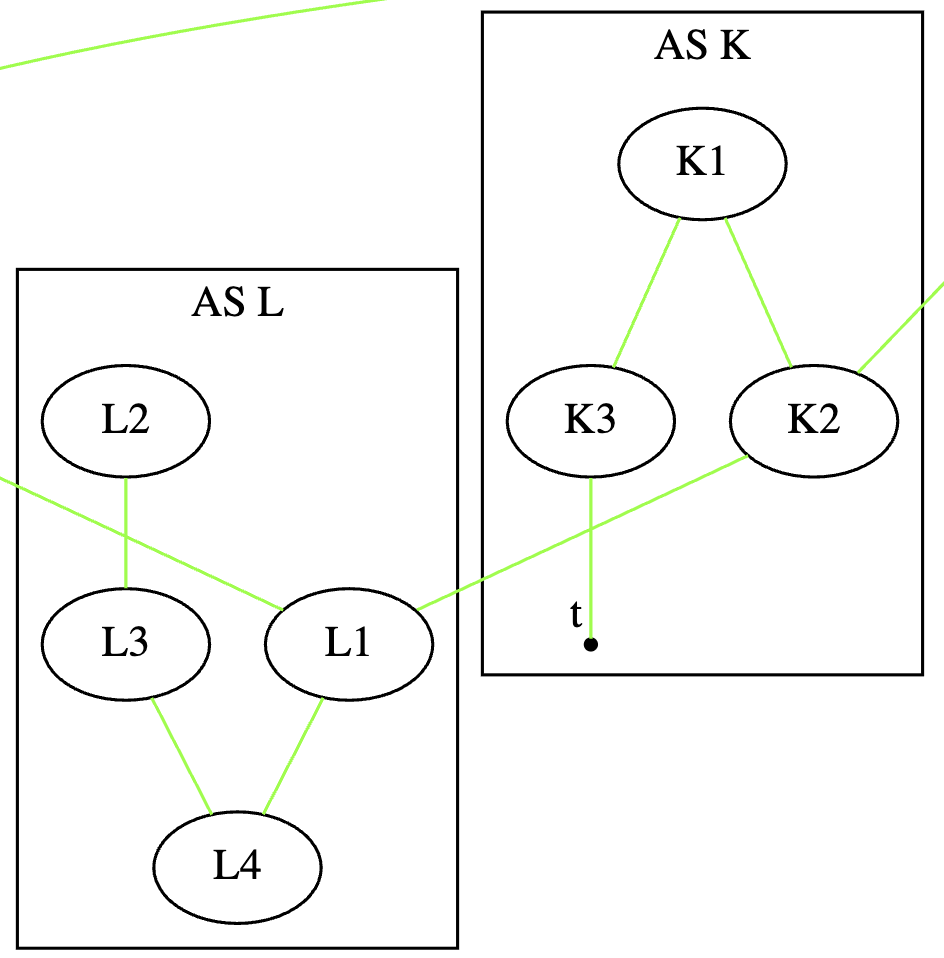
\includegraphics[width=\textwidth]{./images/m05-l06-1.png}
    \end{minipage}
\end{theorem}

\begin{theorem}
    {Route aggregation in BGP}

    \begin{itemize}
        \item Reduces size of routing table
        \item Reduce number of advertisements
    \end{itemize}
\end{theorem}

\subsubsection{Routing between ASes}

\begin{theorem}
    {Hot potato routing}
    Hands off packet to neighboring AS as quickly as possible to minimize cost within own AS.

    Steps for A to update its forwarding table to reach host B in another AS:
    \begin{enumerate}
        \item Learn from inter-AS protocol that the network containing host B is reachable through multiple border routers
        \item Use routing info from intra-AS protocol to determine least-cost path to each border router
        \item Choose border router with lowest-cost path
        \item Determine from forwarding table the interface that leads to least-cost border router
        \item Enter network of B and corresponding interface in forwarding table
    \end{enumerate}
\end{theorem}

\begin{knBox}
    {BGP Route Hijacking: MITM attack}
\end{knBox}

\sectionbar{M05-L06}

\subsection{Network Address Translation}

\begin{definition}
    {Network Address Translation (NAT)}

    \begin{itemize}
        \item Private IP addresses are not routable on the internet
        \item Has a \textbf{translation table} to keep track of active connections. Tuple of \texttt{(internal IP:port, remote IP:port, protocol, NAT IP:port)}
        \item NAT assigns a unique port number for each outgoing connection from an internal host to the external network.
        \item NAT \textbf{simply changes} the destination IP address and port of the packet, leaving the size and payload unchanged.
        \item When response is received, NAT finds the corresponding tuple \texttt{(remote IP, remote port, protocol, NAT port)} in its translation table to forward the packet to the correct internal host.
        \item To handle having a server inside a private network, \textbf{port forwarding / (UPnP)} can be used to map a specific port on the public IP address to a specific internal IP address and port.
        \item Works for \textit{transport protocols} like TCP and UDP as well
    \end{itemize}


    \begin{tabular}{l|l|l}
        \textbf{Stage}            & \textbf{Source IP : Port}  & \textbf{Destination IP:Port} \\ \hline
        Packet leaving host       & Unchanged (host)           & Unchanged                    \\
        Packet leaving NAT router & NAT IP : Assigned NAT port & Unchanged                    \\
        Packet leaving remote     & Unchanged (remote)         & NAT IP : Assigned NAT port   \\
        Remote host packet        & Unchanged (remote)         & NAT IP : Mapped port         \\
    \end{tabular}

\end{definition}
Advantages:
\begin{itemize}
    \item Hide the internal source and destination of packets from a network observer.
    \item Scale IP addresses to more than 4 billion devices.
    \item Can change your ISP without changing the IP addresses of the end hosts.
\end{itemize}

Disadvantages:
\begin{itemize}
    \item NAT increases the time taken for a router to forward a packet
    \item Routers require larger memory to store address translations.
\end{itemize}

\sectionbar{M06-L01}